% Secondo periodo
\subsubsection{Secondo periodo (27/11/2023 - 12/12/2023)}

\subsubsubsection{Planning}
\subsubsubsubsection*{Attività pianificate}
All'inizio del periodo ad ogni membro del gruppo sono stati assegnati ruoli specifici, di seguito riportati:
\begin{table}[H]
\centering
\begin{tabular}{|c|c|c|}
\hline
\textbf{Membro} & \textbf{Ruolo} \\
\hline
Samuele V. & Responsabile \\
\hline
Michele Z. & Analista \\
\hline
Leonardo B. & Analista \\
\hline
Riccardo Z. & Programmatore \\
\hline
Filippo T. & Verificatore \\
\hline
Davide B. & Amministratore \\
\hline
\end{tabular}
\caption{Ruoli assunti per ciascun membro del team all'inizio del periodo}
\end{table}
Si è deciso di non coinvolgere il ruolo di "Progettista"  e, invece, di introdurre il ruolo di ”Programmatore” come figura che, almeno nelle prime fasi di vita del progetto, si occuperà della stesura dei verbali e altri documenti.

Gli obiettivi posti per lo sprint sono stati i seguenti:
\begin{itemize}
    \item Approfondire con il proponente le tecnologie da utilizzare;
    \item Cominciare la stesura del documento \emph{Piano di Progetto};
    \item Continuare la stesura del documento \emph{Analisi dei Requisiti};
    \item Approfondire i linguaggi e librerie emersi dall'ultimo incontro con il proponente:
    \begin{itemize}
        \item \emph{Javascript};
        \item \emph{React};
        \item \emph{Docker}.
    \end{itemize}
    \item Approfondire con il proponente alcune questioni emerse sul documento di \emph{Analisi dei Requisiti};
\end{itemize}

\subsubsubsubsection*{Preventivo}
\begin{table}[H]
    \centering
\begin{spreadtab}{{tabular}{|c|c|c|c|c|c|c|c|}}
    \hline
    @\textbf{Membro} & @\textbf{Re} & @\textbf{Amm} & @\textbf{An} & @\textbf{Progr} & @\textbf{Proge} & @\textbf{Ve} & @\textbf{Totale} \\
    \hline
    @ Samuele V.   & 4          & 0          & 0         & 0          & 0     & 1     & sum(b2:g2) \\
    @ Leonardo B.  & 0         & 0          & 3        & 0        & 0     & 0    & sum(b3:g3) \\
    @ Riccardo Z.  & 0          & 0          & 0          & 4          & 0     & 0   & sum(b4:g4) \\
    @ Davide B.    & 0          & 4          & 0       & 0       & 0     & 0     & sum(b5:g5) \\
    @ Michele Z.   & 0          & 0          & 3         & 0          & 0     & 0     & sum(b6:g6) \\
    @ Filippo T.   & 0          & 0          & 0         & 0          & 0     & 4     & sum(b7:g7) \\
    \hline
    @\textbf{Ore totali} & sum(b2:b7) & sum(c2:c7) & sum(d2:d7) & sum(e2:e7) & sum(f2:f7) & sum(g2:g7) &  sum(b8:g8)\\
    \hline
    @\textbf{Costo totale} & 30*b8 & 20*c8 & 25*d8 & 15*e8 & 25*f8 & 15*g8 & sum(b9:g9)\\
    \hline
\end{spreadtab}
    \caption{Preventivo orario ed economico parziale per il secondo periodo, in base al ruolo}
    \label{tab:prev_rtb}
    \vspace{5mm}
    \textbf{Legenda:} \textit{Re} = Responsabile, \textit{Amm} = Amministratore, \textit{An} = Analista, \textit{Progr} = Programmatore, \textit{Proge} = Progettista, \textit{Ve} = Verificatore
\end{table}


\begin{figure}[H]
  \centering
  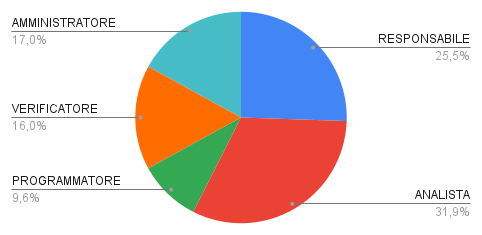
\includegraphics[width=0.6\linewidth]{grafici/2_periodo_torta.png}
  \caption{Ripartizione dei costi per ruolo nel $2^\circ$ periodo}
        \vspace{10mm}
  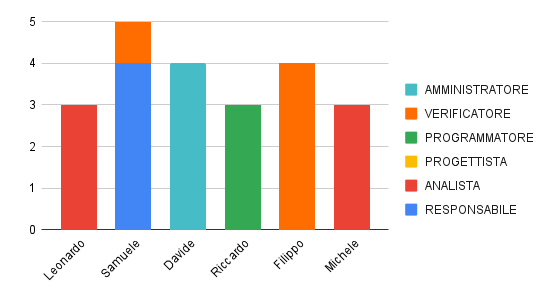
\includegraphics[width=0.7\linewidth]{grafici/2_periodo_istogramma.png}
  \caption{Ore preventivate per ciascuna persona nel $2^\circ$ periodo}
\end{figure}



\subsubsubsection{Review}
\subsubsubsubsection*{Attività svolte}
Le attività preventivate sono state svolte con successo e sono state le seguenti:
\begin{itemize}
    \item E' stato continuato il documento \emph{Analisi Dei Requisiti};
    \item E' stato continuato il documento \emph{Norme di Progetto};
    \item E' stato effettuato dello studio individuale di \emph{Javascript} e \emph{React};
    \item E' stato effettuato un incontro con il proponente durante il quale:
    \begin{itemize}
        \item Sono stati chiariti dubbi sugli scenari secondari di alcuni casi d'uso;
        \item E' stato proposto con successo un timer entro lo scadere del quale è possibile fare le modifiche all'ordinazione collaborativa;
        \item E' stato consigliato l'utilizzo dei framework \emph{Bootstrap} e di \emph{NextJS}.
    \end{itemize}
\end{itemize}
\subsubsubsubsection*{Consuntivo}
\begin{table}[H]
    \centering
\begin{spreadtab}{{tabular}{|c|c|c|c|c|c|c|c|}}
    \hline
    @\textbf{Membro} & @\textbf{Re} & @\textbf{Amm} & @\textbf{An} & @\textbf{Progr} & @\textbf{Proge} & @\textbf{Ve} & @\textbf{Totale} \\
    \hline
    @ Samuele V.   & 3          & 0          & 0         & 0          & 0     & 1     & sum(b2:g2) \\
    @ Leonardo B.  & 0         & 0          & 4        & 0        & 0     & 0    & sum(b3:g3) \\
    @ Riccardo Z.  & 0          & 0          & 0          & 3          & 0     & 0   & sum(b4:g4) \\
    @ Davide B.    & 0          & 3          & 0       & 0       & 0     & 0     & sum(b5:g5) \\
    @ Michele Z.   & 0          & 0          & 3         & 0          & 0     & 0     & sum(b6:g6) \\
    @ Filippo T.   & 0          & 0          & 0         & 0          & 0     & 3     & sum(b7:g7) \\
    \hline
    @\textbf{Ore totali} & sum(b2:b7) & sum(c2:c7) & sum(d2:d7) & sum(e2:e7) & sum(f2:f7) & sum(g2:g7) &  sum(b8:g8)\\
    \hline
    @\textbf{Costo totale} & 30*b8 & 20*c8 & 25*d8 & 15*e8 & 25*f8 & 15*g8 & sum(b9:g9)\\
    \hline
   % @\textbf{Diff. preventivo} & 0 & 0 & 0 & 0 & 0 & 0 & sum(b10:g10)\\
   % \hline
\end{spreadtab}
    \caption{Consuntivo orario ed economico parziale per il secondo periodo, in base al ruolo}
    \label{tab:prev_rtb}
    \vspace{5mm}
    \textbf{Legenda:} \textit{Re} = Responsabile, \textit{Amm} = Amministratore, \textit{An} = Analista, \textit{Progr} = Programmatore, \textit{Proge} = Progettista, \textit{Ve} = Verificatore
\end{table}
\subsubsubsection{Retrospective}

I rischi verificati in questa fase sono stati:\nameref{ro:1},\nameref{ro:4}.
Dal punto di vista organizzativo ci sono stati diversi problemi. Inoltre sono emersi diversi dubbi riguardanti la stesura del documento di \emph{Analisi dei Requisiti}.
In particolare, sono sorti durante l'uso degli USE CASE. Infine ci sono stati dei dubbi riguardo la verifica dello stato di avanzamento dei lavori e su come individuare in quali ambiti si stanno riscontrando criticità.
In particolare sono emerse le seguenti criticità:
\begin{itemize}
    \item Lo scarso utilizzo fino al quel momento di scenari secondari;
    \item Dubbi sulla gestione di eventuali scenari che potrebbero riguardare casi d’uso principali o sotto casi;
    \item Dubbi riguardanti casi d’uso che coinvolgono più attori contemporaneamente;
    \item Dubbi riguardanti l'utilizzo della locuzione \emph{extend}.
\end{itemize}
Per mitigare tali problemi si è ideato un documento interno che riguarda i pattern da seguire per stilare il documento di Analisi dei Requisiti.